\section{Results}
\label{section:results}

In order to demonstrate the performance of our method, we conducted two sets
of tests.
In the first we simulated a set of observables from a set fundamental
parameters for a few hundred stars using the MIST stellar evolution models and
a gyrochronology model, then compared the parameters predicted with our model
to the true parameters used to generate the data.
In the second we tested our model by attempting the measure the ages of
individual stars in the Praesepe open cluster and compared the results to the
establised age of Praesepe.
The age of Praesepe, like any open cluster, has been measured precisely
because it is an ensemble of coeval stars with the same metallicity: a single
stellar poplulation, and its age can be precisely established through
isochrone fitting and MS turn-off.
We adopted an age of 650 Myrs for Praesepe \citep{fossati2008, perryman1998}.

\subsection{Test 1: simulated stars}
For the first test we drew masses, ages, bulk metallicities, distances and
extinctions at random for 1000 stars from the following uniform distributions:
\begin{eqnarray}
& M \sim U(0.5, 1.5)~[M_\odot] \\
& A \sim U(0.5, 14)\mathrm{~[Gyr]} \\
& F \sim U(-0.2, 0.2) \\
& D \sim U(10, 1000)~\mathrm{[pc]} \\
& A_V \sim U(0, 1).
\end{eqnarray}
\teff, \logg, \fhat, \pmega\, $C_{B-V}$ and apparent magnitudes $J$, $H$ and
$K$ were generated, without noise, from these stellar parameters using the
MIST stellar evolution models.
Rotation periods were generated using the gyrochronology relation of
equation \ref{eqn:gyro}.
We took two approaches to inferring the ages of these simulated stars:
firstly using isochrone fitting {\it only}, and secondly using isochrone
fitting {\it combined with} a gyrochronology model.
For all stars, our initial guesses for the parameters were $M = 1M_\odot$,
$A = 1$ Gyr, $F = 0$, $D = 500$ pc and $A_V = 0.1$.

%   - The results
Figure \ref{fig:iso_only} shows the results of using isochrone fitting
to estimate the posterior PDFs over the stellar ages of simulated stars.
True stellar ages are plotted on the $x$-axis and the posterior PDFs of the
inferred ages are plotted on the $y$-axis.
The rotation periods of stars were not incorporated into this model: these
posterior PDFs were obtained by isochrone fitting only, using the likelihood
function in equation \eqref{eqn:isochrones_only_likelihood}.
In most cases ages are only weakly constrained by the stellar evolution models
and in some cases there is no age constraint: the age of the star is
consistent with all ages from 0-14 Gyrs.
This is because stellar temperatures and luminosities do not change rapidly on
the main sequence: isochrones are tightly spaced there and, as a result, even
precisely measured temperatures and luminosities often do not yield precise
ages.
Figure \ref{fig:iso_and_gyro} shows the results of using isochrones {\it
combined} with a gyrochronology model.
These ages were inferred using the likelihood of equations
\eqref{eqn:full_likelihood}/\eqref{eqn:both_likelihood}.
Again, figure \ref{fig:iso_and_gyro} shows true stellar ages on the $x$-axis
and the posterior PDFs of the inferred ages on the $y$-axis.
Here, unlike the isochrone only case, the recovered ages are precise because
there is more age information in stellar rotation periods than in effective
temperatures and absolute magnitudes.
Gyrochronology isochrones (or gyrochrones) are more widely separated relative
to the observational uncertainties than the MIST isochrones.
Put another way, the rotation periods of two stars of different ages and the
same mass will have rotation periods that differ significantly -- almost
certainly more than the observational uncertainty on rotation period.
On the other hand, such stars are likely to have extremely similar
luminosities and temperatures and the differences between these properties are
likely to be smaller than the observational uncertainties.

Figures \ref{fig:iso_precision} and \ref{fig:gyro_precision} show the
simulated stars on a color magnitude diagram, colored by the relative
precision of their predicted ages.
Figure \ref{fig:iso_precision} shows age precision as a function of CMD
position using isochrone fitting only, and figure \ref{fig:gyro_precision}
shows age precision using isochrone fitting and gyrochronology combined.
These figures are semi-empirical versions of figures \ref{iso_fisher} and
\ref{gyro_fisher}, which were created using information theory, and show the
theoretical minimum precision of isochrone fitting and gyrochronology.
\racomment{Still to do: add these figures!}

% We're cheating here.
% Figure \ref{gyro_only} demonstrates the results of inferring ages using
% rotation periods only, and this illustrates why the combination of isochronal
% and gyrochronal ages is so precise: almost all this precision comes from
% rotation periods.
This simulation experiment is unrealistic for two main reasons: firstly, we
simulated data from the same gyrochronology model we used to infer ages and so
the results will be perfectly accurate by design.
Secondly, we simulated data without any intrinsic scatter built into the
gyrochronology model; it is a deterministic model.
This means that a rotation period and color predicts a corresponding
single-valued age, rather than a probability distribution over ages.
This is unrealistic given observations of open clusters whose members clearly
show excess scatter in their rotation periods, particularly for less massive
stars (see figure \ref{fig:praesepe}).
These results look precise and accurate, but this is misleading.
Inaccuracies would arise if the gyrochronology model was incorrect or poorly
calibrated in some areas of parameter space and imprecision would arise if
intrinsic scatter were built into the gyrochronology model and/or the
observations.
The result of using a deterministic model, such as the one used in this
experiment, is that the uncertainties on stellar ages will be unrealistically
small.
We leave the recalibration of gyrochronology models for a future exercise
since, in this work, we are mostly interested in testing the results of simply
combining gyrochronology and isochrone fitting.
The above experiment shows that building gyrochronology into stellar evolution
models results in much more precise age predictions, as predicted by
information theory.
We have not yet made any statement about accuracy however; the above
experiment produces accurate ages by construction.
In order to test the accuracy of this method, we tested it on real data: the
Praesepe open cluster.

% TEST 2: Clusters
%-----------------------------------------------------------------------------
%   - The cluster data
\subsection{Test 2: the Praesepe Cluster}
In order to test our model on real stars with known ages, we selected a sample
of cluster stars with precisely measured ages from ensemble isochrone fitting
and main sequence turn off.
The ages of open clusters can be measured much more precisely than field
stars.
Stars in the same cluster formed (we assume) from the same molecular cloud at
the same time and therefore have the same metallicity and age (to within a few
million years).
Stars with the same metallicity and age fall on the same isochrone,
allowing perfect isochrone selection and providing a $N^{-1/2}$ decrease in
uncertainty where N is the number of cluster stars.
Single stellar populations also allow main sequence turn off to be identified
and, as demonstrated in figure \ref{fig:iso_fisher}, the turn off supplies a
large amount of age information.
We compiled rotation periods, \Gaia\ photometry and \gaia\ parallaxes for
members of Praesepe, a $\sim$650 Myr cluster \citep{fossati2008}.
We chose Praesepe because it is relatively tightly clustered on the sky and
many of its members were targeted in a single \ktwo\ campaign, from which it
was possible to measure rotation periods via frequency analysis of member's
light curves \citep{douglas2017}.
We crossmatched Praesepe members with measured rotation periods
\citep{douglas2017} with the Gaia DR2 catalog \citep{brown2018}, using a 1''
search radius.
The result was a sample of 757 stars with rotation periods, parallaxes and
\gaia\ $G$, $G_{BP}$ and $G_{RP}$-band photometry.
Figure \ref{fig:praesepe} shows the rotation periods of Praesepe members as
a function of their \gaia\ \gcolor\ colors.
The GK and early M dwarfs (\gcolor\ $<$ 2.4) which fall on a `rotational main
sequence' are shown as blue points and the late M dwarfs (\gcolor\ $>$ 2.4)
whose rotation periods are not well determined by their age and color are
shown as orange open circles.
We excluded the late M dwarfs (orange circles with \gcolor\ $>$ 2.4) from this
analysis since they do not follow a simple gyrochronology relation however, we
included more massive outliers (orange circles with \gcolor\ $<$ 2.4) in order
to provide a complete picture of the precision and accuracy of gyrochronology
applied to Praesepe.
Figure \ref{fig:praesepe} shows two sets of gyrochronology models: one
calibrated using several open clusters, asteroseismic stars and the Sun
\citep{angus2015}, which was used to infer the ages of Praesepe but clearly
does not provide a perfect fit to this cluster (solid gray line), and one fit
to Praesepe and the Sun only, as described in section
\ref{section:motivation}, that was used to calculate the Fisher information
(dashed black line).
We did not account for extinction in our analysis since Praesepe is relatively
nearby (around 180 parsecs) so reddening from dust is minimal.

% The age of each Praesepe member was inferred using both of these
% gyrochronology models: the legacy model of equation \ref{eq:gyro} and the
% Praesepe model of equation \ref{eq:new_gyro}.
% This exercise is not designed to test one gyrochronology model against
% another: the model fit to the Praesepe data will provide a better age
% prediction by design, as the legacy model was fit to number of clusters at
% once.
% The point of this exercise is to show how precise gyrochronology could be if
% a {\it perfect} model was used.
% The age of each Praesepe member was inferred using our combined stellar
% evolution and gyrochronology model.
% We did not force the cluster members to have the same age since the aim of
% this experiment was to reveal the precision and accuracy of our method by
% quantifying the level of scatter in our predicted ages and identifying regions
% of parameter space where the ages deviate from the established age for
% Praesepe.

%   - Praesepe results: ages
The resulting probability density functions over age predicted for individual
members of Praesepe, where each member was treated as an isolated field star,
are shown in figure \ref{fig:ages}.
The orange distributions show posterior PDFs over age for each member of
Praesepe, where ages were inferred using isochrone fitting {\it only},
with \gaia\ colors (\gcolor), \gaia\ apparent magnitude ($G$), and \gaia\
parallaxes as the observable properties.
The blue distributions are posterior PDFs over stellar age for each member of
Praesepe, where ages were inferred using isochrone fitting {\it and}
a gyrochronology model (equation \ref{eqn:gyro}).
The blue posteriors are much more strongly peaked around the literature age of
the cluster (650 Myrs, indicated by a vertical black line) and this
demonstrates that rotation periods carry far more age information than
photometric colors, even when precise parallaxes are available.

% % Cutting outliers and limiting color range.
% In order to fit a period-color relation to these data we restricted the sample
% of cluster stars to the color range, 0.56 $<$ \gcolor\ $<$ 3 in order to
% remove early F and late M dwarfs whose rotation periods do not fall on the
% `gyrochronology main sequence'.
% Although it {\it may} be possible to crudely predict the ages of these stars
% (at least the M dwarfs) from their rotation periods, the age-rotation-color
% relation for these stars is very different to the FGK star relations and is
% not the focus of this paper.
% In addition, we removed rapidly rotating stars from the sample since, although
% modeling outliers is important and consequential for gyrochronology in
% general, the goal of this paper is not to produce a perfect gyrochronology
% that reproduces stochasticity in the data, just a simple function that fits
% the rotational main sequence of Praesepe.
% In future we plan to update the gyrochronology models to include M dwarfs,
% and the outlying rapid rotators using a mixture of Gaussians.
% Similarly, we used only Praesepe in this study because the period-color
% relations of each open cluster with rotation periods has a different shape.
% This is likely due to differences in metalicities, incomplete or noisy
% membership lists and differences in rotation period measurement algorithms.
% A global gyrochronology calibration, using all cluster data is planned for the
% future but, again, is beyond the scope of the project presented here.
% The rotation periods of the Praesepe members in the restricted color range and
% with outliers removed are plotted against their \Gaia\ colors in figure
% \ref{fig:Praesepe}.
% We used linear least squares to fit a linear model to Praesepe and the Sun.
% A 4th order polynomial in $\log(G_{BP} - G_{RP})$ and a straight line in
% $\log(\mathrm{Age~[yrs]})$ was fit to reproduce
% $\log(\mathrm{rotation~period~[days]})$.
% \begin{equation}
%     \log(P) = a + b\log(C_G) + c\log^2(C_G) + d\log^3(C_G) + e\log^4(C_G) +
%     f\log(A),
% \end{equation}
% \label{eq:new_gyro}
% were $P$ is period, $C_G$ is \Gaia \gcolor\ color, and A is age.

% %   - Praesepe results: metallicity, mass, distance
% Stellar rotation periods are age-informative and so including them in our
% analysis leads to the more precise measurement of ages.
% However, rotation periods do not carry very much information about the
% metallicity of a star, nor their distance.
% They are also not particularly informative about the mass of a star because,
% even though rotation period depends on both mass and age, stellar mass is
% strongly informed by color and temperature information, so is chiefly
% determined by the stellar evolution/isochrone models.
% However, age, mass and metallicity are correlated: a star can be more blue
% because it is more massive, older or more metal poor and for this reason, if a
% star's age is more tightly constrained, constraints on its mass and
% metallicity will also improve.
% Figures \ref{fig:metallicity} and \ref{fig:mass} show the differences in
% posterior PDFs over metallicity and mass respectively, calculated for Praesepe
% stars where rotation period information is both used (blue posteriors) and not
% used (orange posteriors).
% The black line in figure \ref{fig:metallicity} shows the established
% metallicity of Praesepe \racomment{citation}.
% There is little difference between blue and orange because rotation periods do
% not strongly depend on metallicity or mass (independantly of age).
% However, the precision of mass and metallicity measurements are slightly
% improved due to the fact that age, mass and metallicity are correlated.
% Figure \ref{fig:distances} shows the posterior PDFs over distance to the
% Praesepe cluster.
% In this example of fitting our model to Prasepe data, Since we used \gaia\
% parallaxes, which are extremely informative about distances, more precisely
% constrained ages make a minimal improvement to distances.

%   - Praesepe results: the Praesepe gyro relation
% The results in figure \ref{fig:praesepe_old_model_ages} were produced using a
% gyrochronology relation (equation \ref{eqn:old_gyro}) that was calibrated
% using the Hyades, Coma Berenices and Pleiades clusters, plus the Sun and old
% asteroseismic stars \citep{angus2015}.
% Figure \ref{fig:praesepe_new_model_ages} however, shows the results of
% inferring the ages of Praesepe members with the dedicated Praesepe
% gyrochronology relation of equation \ref{eqn:gyro_age_praesepe}.
% We include these results because we would like to provide an idea of the kind
% of age measurement accuracy that is achievable in the best case: where the
% gyrochronology model perfectly reproduces the data.

%   - Summary
In summary, fitting our new age model to simulated stars and members of the
Praesepe cluster (an open cluster with a precisely measured age from ensemble
isochrone fitting and MS turn-off) demonstrates that using isochrone fitting
{\it alone} to calculate the ages of cool MS field stars results in
extremely imprecise ages, however when gyrochonology is incorporated, the
precision of age measurements increase significantly.

% The simulation figures
% iso only
\begin{figure}
  \caption{
The results of a test in which we simulated observable properties of stars
    with the same model we used to infer their properties.
In this experiment we used {\it only} isochrone fitting to infer ages;
we did not use rotation periods/gyrochronology.
    For results where we used {\it both} stellar evolution models {\it and}
    gyrochronology, see figure \ref{fig:iso_and_gyro}.
The true age, used to produce associated observables is shown on the x-axis,
    and the inferred ages are shown on the y-axis.
This figure shows the posterior PDFs over stellar age for each of the
    simulated stars as a `violin plot', where samples from the posterior are
    plotted vertically as a smooth, symmetric function.
The widths of these functions indicates the probability density over age:
    wider regions indicated greater probability mass.
The median values of the posterior PDFs are plotted as solid horizontal lines.
This figure demonstrates that when only stellar evolution models are used to
    infer ages for field MS stars, the resulting predicted ages are extremely
    imprecise.
}
  \centering
    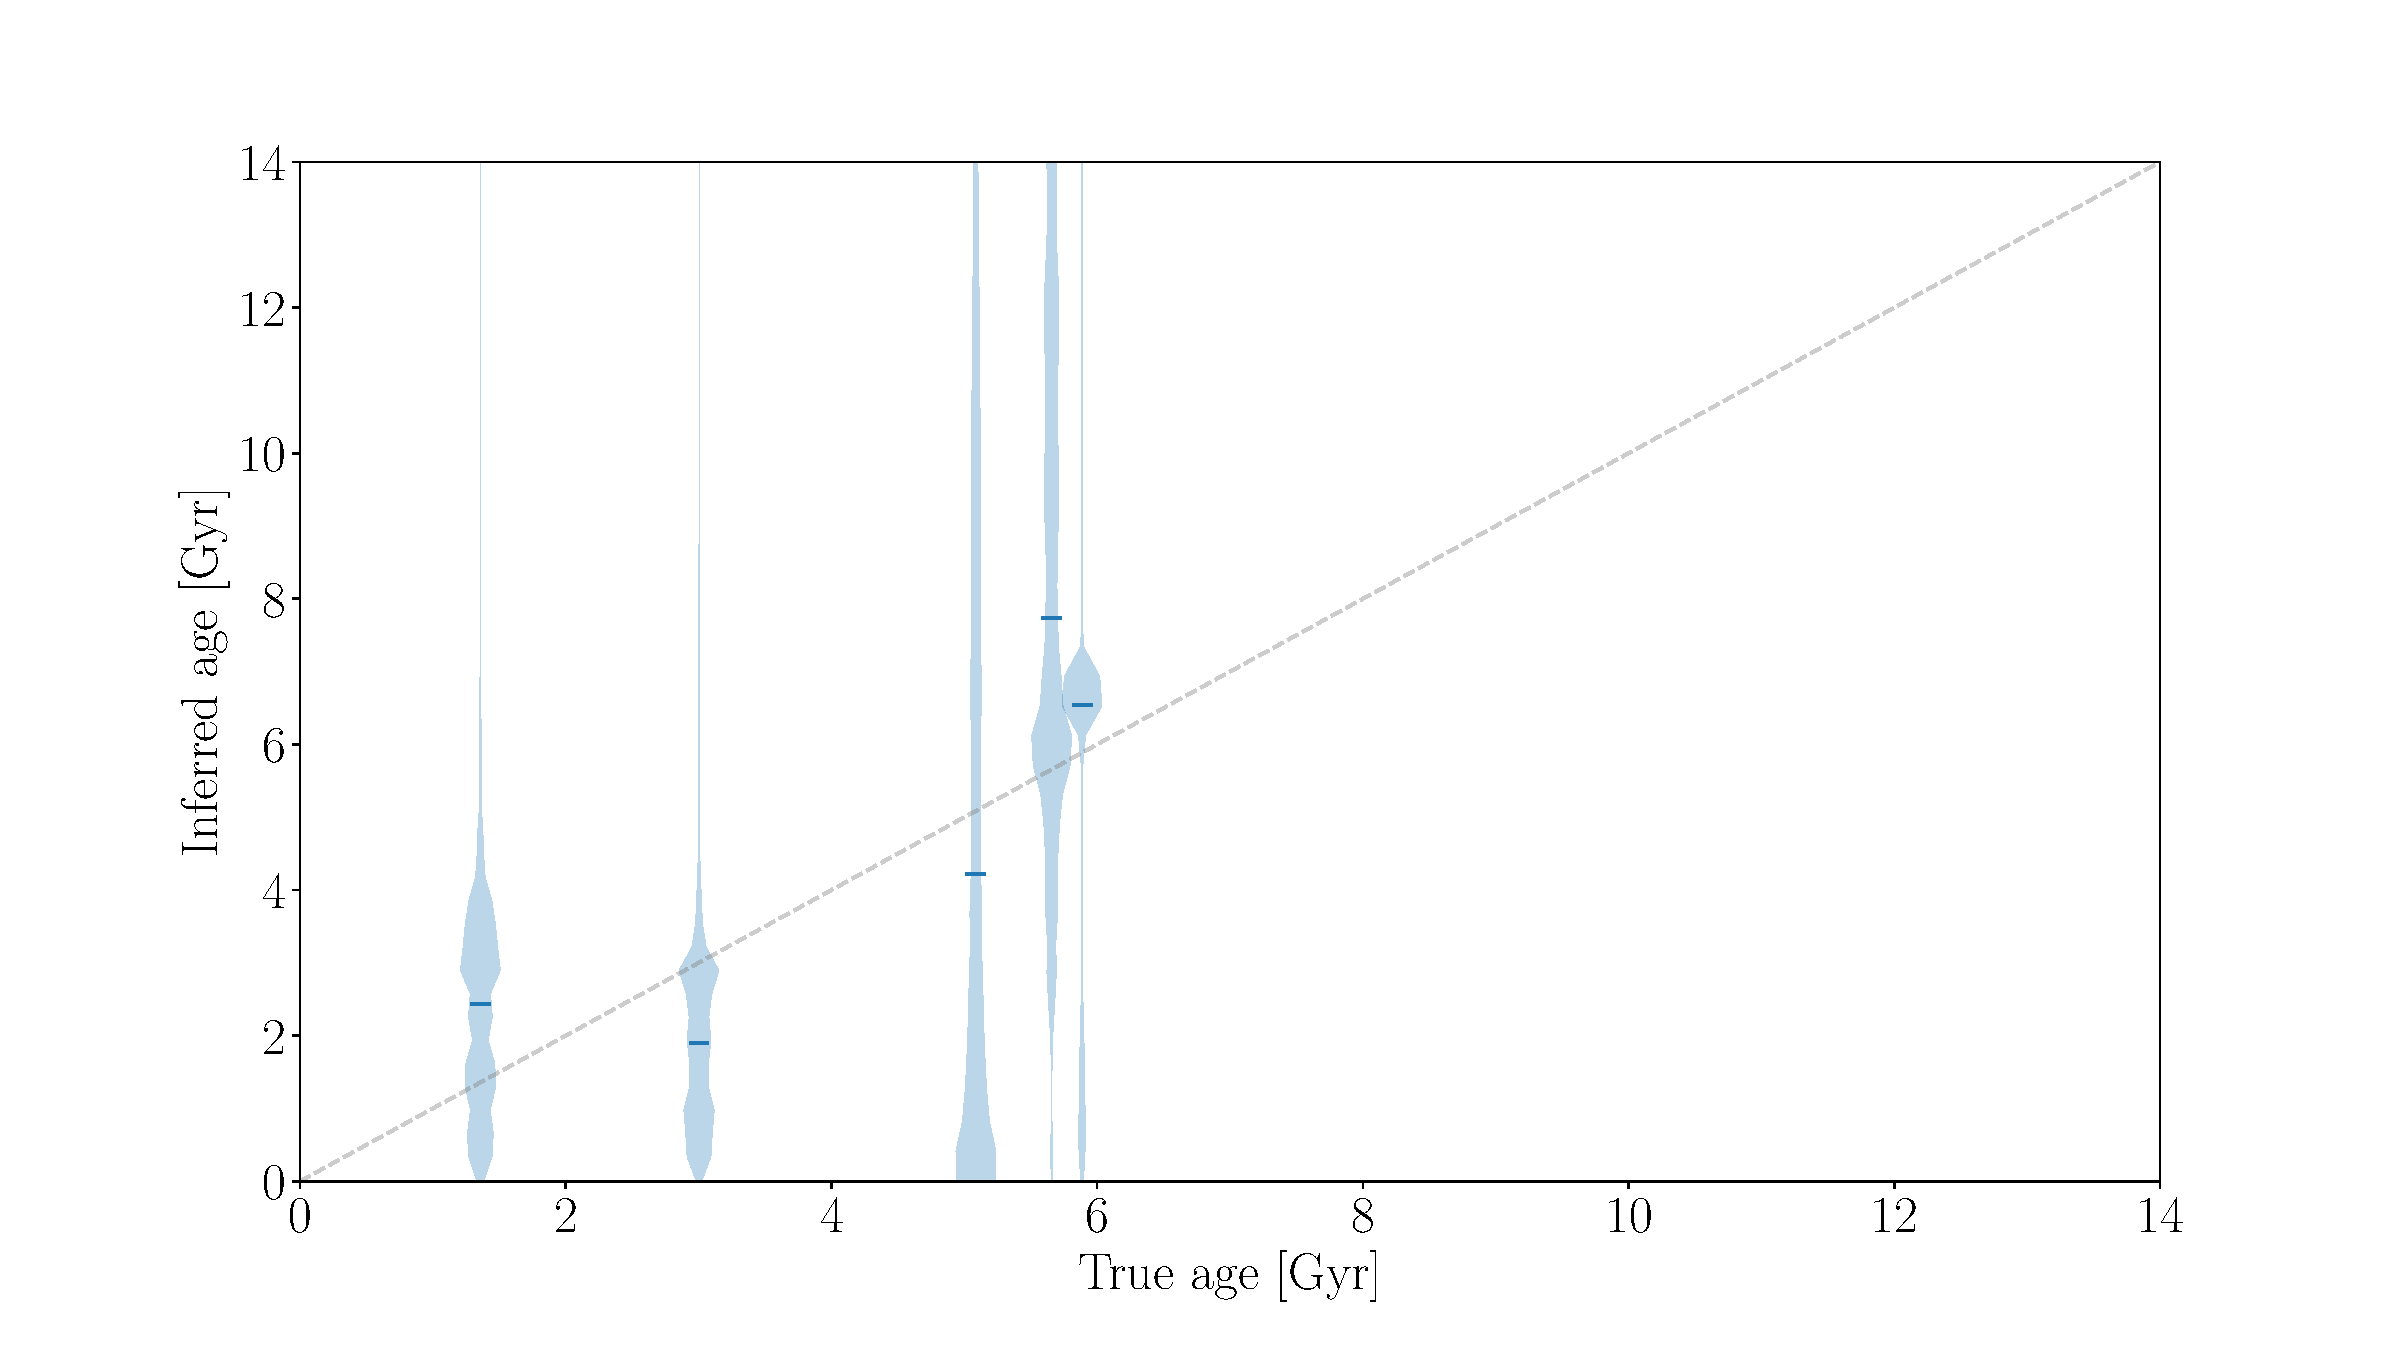
\includegraphics[width=1\textwidth]{../plots/iso_only_violin.pdf}
\label{fig:iso_only}
\end{figure}

\begin{figure}
  \caption{
The results of a test in which we simulated observable properties of stars
    with the same model we used to infer their properties.
    In this experiment we used both isochrone fitting {\it and}
    gyrochronology to infer ages.
For results where we used stellar evolution models {\it only}, see the
    previous figure (figure \ref{fig:iso_only}).
The true age, used to produce associated observables is shown on the x-axis,
    and the inferred ages are shown on the y-axis.
This figure shows the posterior PDFs over stellar age for each of the
    simulated stars as a `violin plot', where samples from the posterior are
    plotted vertically as a smooth, symmetric function.
The widths of these functions indicates the age probability density: wider
    regions represent greater probability mass.
The median values of the posterior PDFs are plotted as solid horizontal lines.
    This figure demonstrates that when rotation periods (gyrochronology) {\it
    and} stellar evolution models are used to infer the ages of field MS
    stars, the resulting predicted ages are much more precise
    than isochrone fitting can provide alone.
    \racomment{I am rerunning code to fix the outliers in this figure -- I
    think it's an initialization issue. I am also planning to combine this
    figure with the figure above.}
}
  \centering
    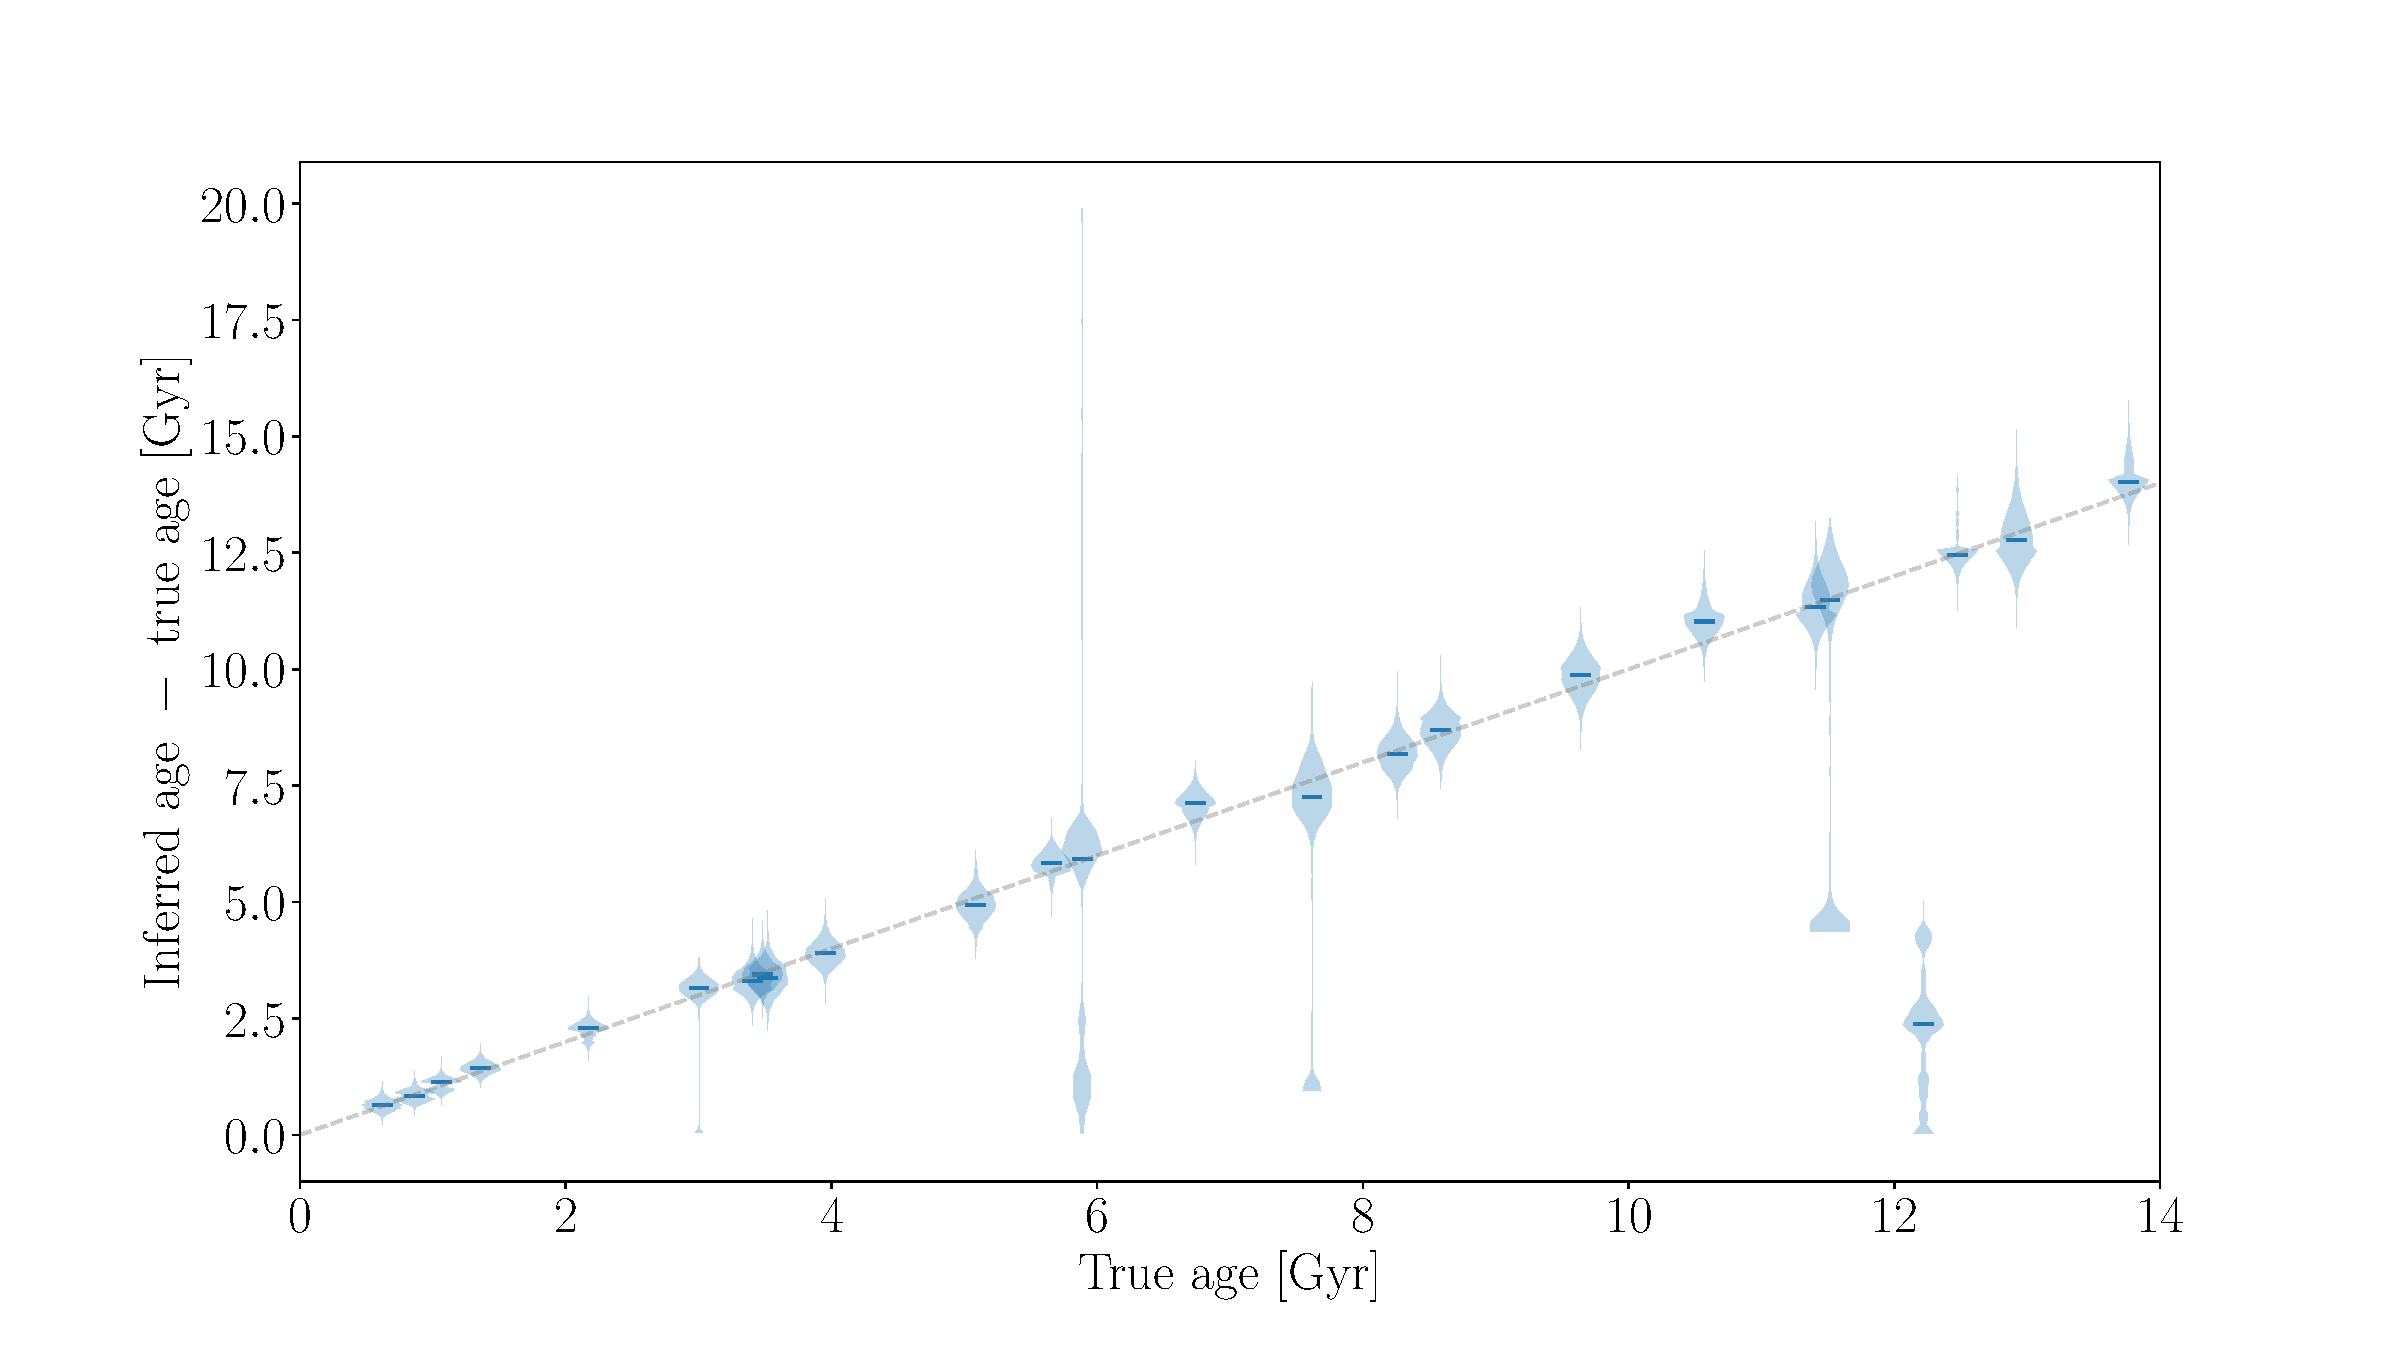
\includegraphics[width=1\textwidth]{../plots/iso_and_gyro_violin.pdf}
\label{fig:iso_and_gyro}
\end{figure}

% % The Cluster figure
% \begin{figure}
%   \caption{
% % The rotation periods of stars in open clusters, and the Sun, plotted against
% %     their \Gaia\ colors (\gcolor) in logarithmic space.
% % The result of this fit is plotted on top of the data at the ages of
% %     the cluster stars and the Sun.
%     The rotation periods of Praesepe members and the Sun, plotted against
%     their \Gaia\ colors (\gcolor) in logarithmic space.
%     We fit a linear model to these data in order to predict
%     rotation periods from \gaia\ colors and age.
%     This model consisted of a fourth-order polynomial in $\log_{10}$ color,
%     and a 1st order polynomial (a straight line) in $\log_{10}$ age.
% The result of this fit is plotted on top of the data at the ages of
%     Praesepe and the Sun.
% }
%   \centering
%     \includegraphics[width=1\textwidth]{clusters.pdf}
% \label{fig:clusters}
% \end{figure}

\begin{figure}
  \caption{
    The rotation periods of Praesepe members \citep{douglas2016}, plotted
    against their \Gaia\ colors (\gcolor) in logarithmic space.
    GK and early M dwarfs (\gcolor\ $<$ 2.4), shown as blue points fall on a
    `rotational main sequence' whereas the rotation periods of late M dwarfs
    (2.4 $<$ \gcolor), shown as orange open circles
    are noisy and not strongly predicted by their age and color.
    We excluded late M dwarfs from our age analysis of Praesepe stars.
    We excluded outliers at earlier spectral types, also shown as open orange
    circles at colors less than 2.4, to perform the polynomial fit to Praesepe
    described in section \ref{section:motivation} (resulting in the black
    dashed line) but included these outliers when inferring the ages of
    Praesepe stars in section \ref{section:results}.
    The early-type outliers were identified via sigma-clipping at
    4.5$\sigma$.
    The black-dashed model was used to calculate the Fisher information shown
    in figures \ref{fig:iso_fisher} and \ref{fig:gyro_fisher}.
    The solid gray lines show gyrochrones that were calibrated using the
    Hyades, Coma Berenices and Pleiades clusters, as well as the Sun and
    \kepler\ asteroseismic stars \citep{angus2015}, and used to predict the
    ages of Praesepe stars, shown in figure \ref{fig:cluster_ages}.
    This model does not provide a perfect fit to Praesepe (Praesepe was not
    used to calibrate it),
    particularly for the hottest and coolest stars,
    however this is the current gyrochronology model implemented in our joint
    isochrone fitting and gyrochronology model.
    This figure was generated in a {\it Jupyter} notebook available at this
    url:
https://github.com/RuthAngus/stardate/blob/master/paper/code/Praesepe.ipynb
}
  \centering
    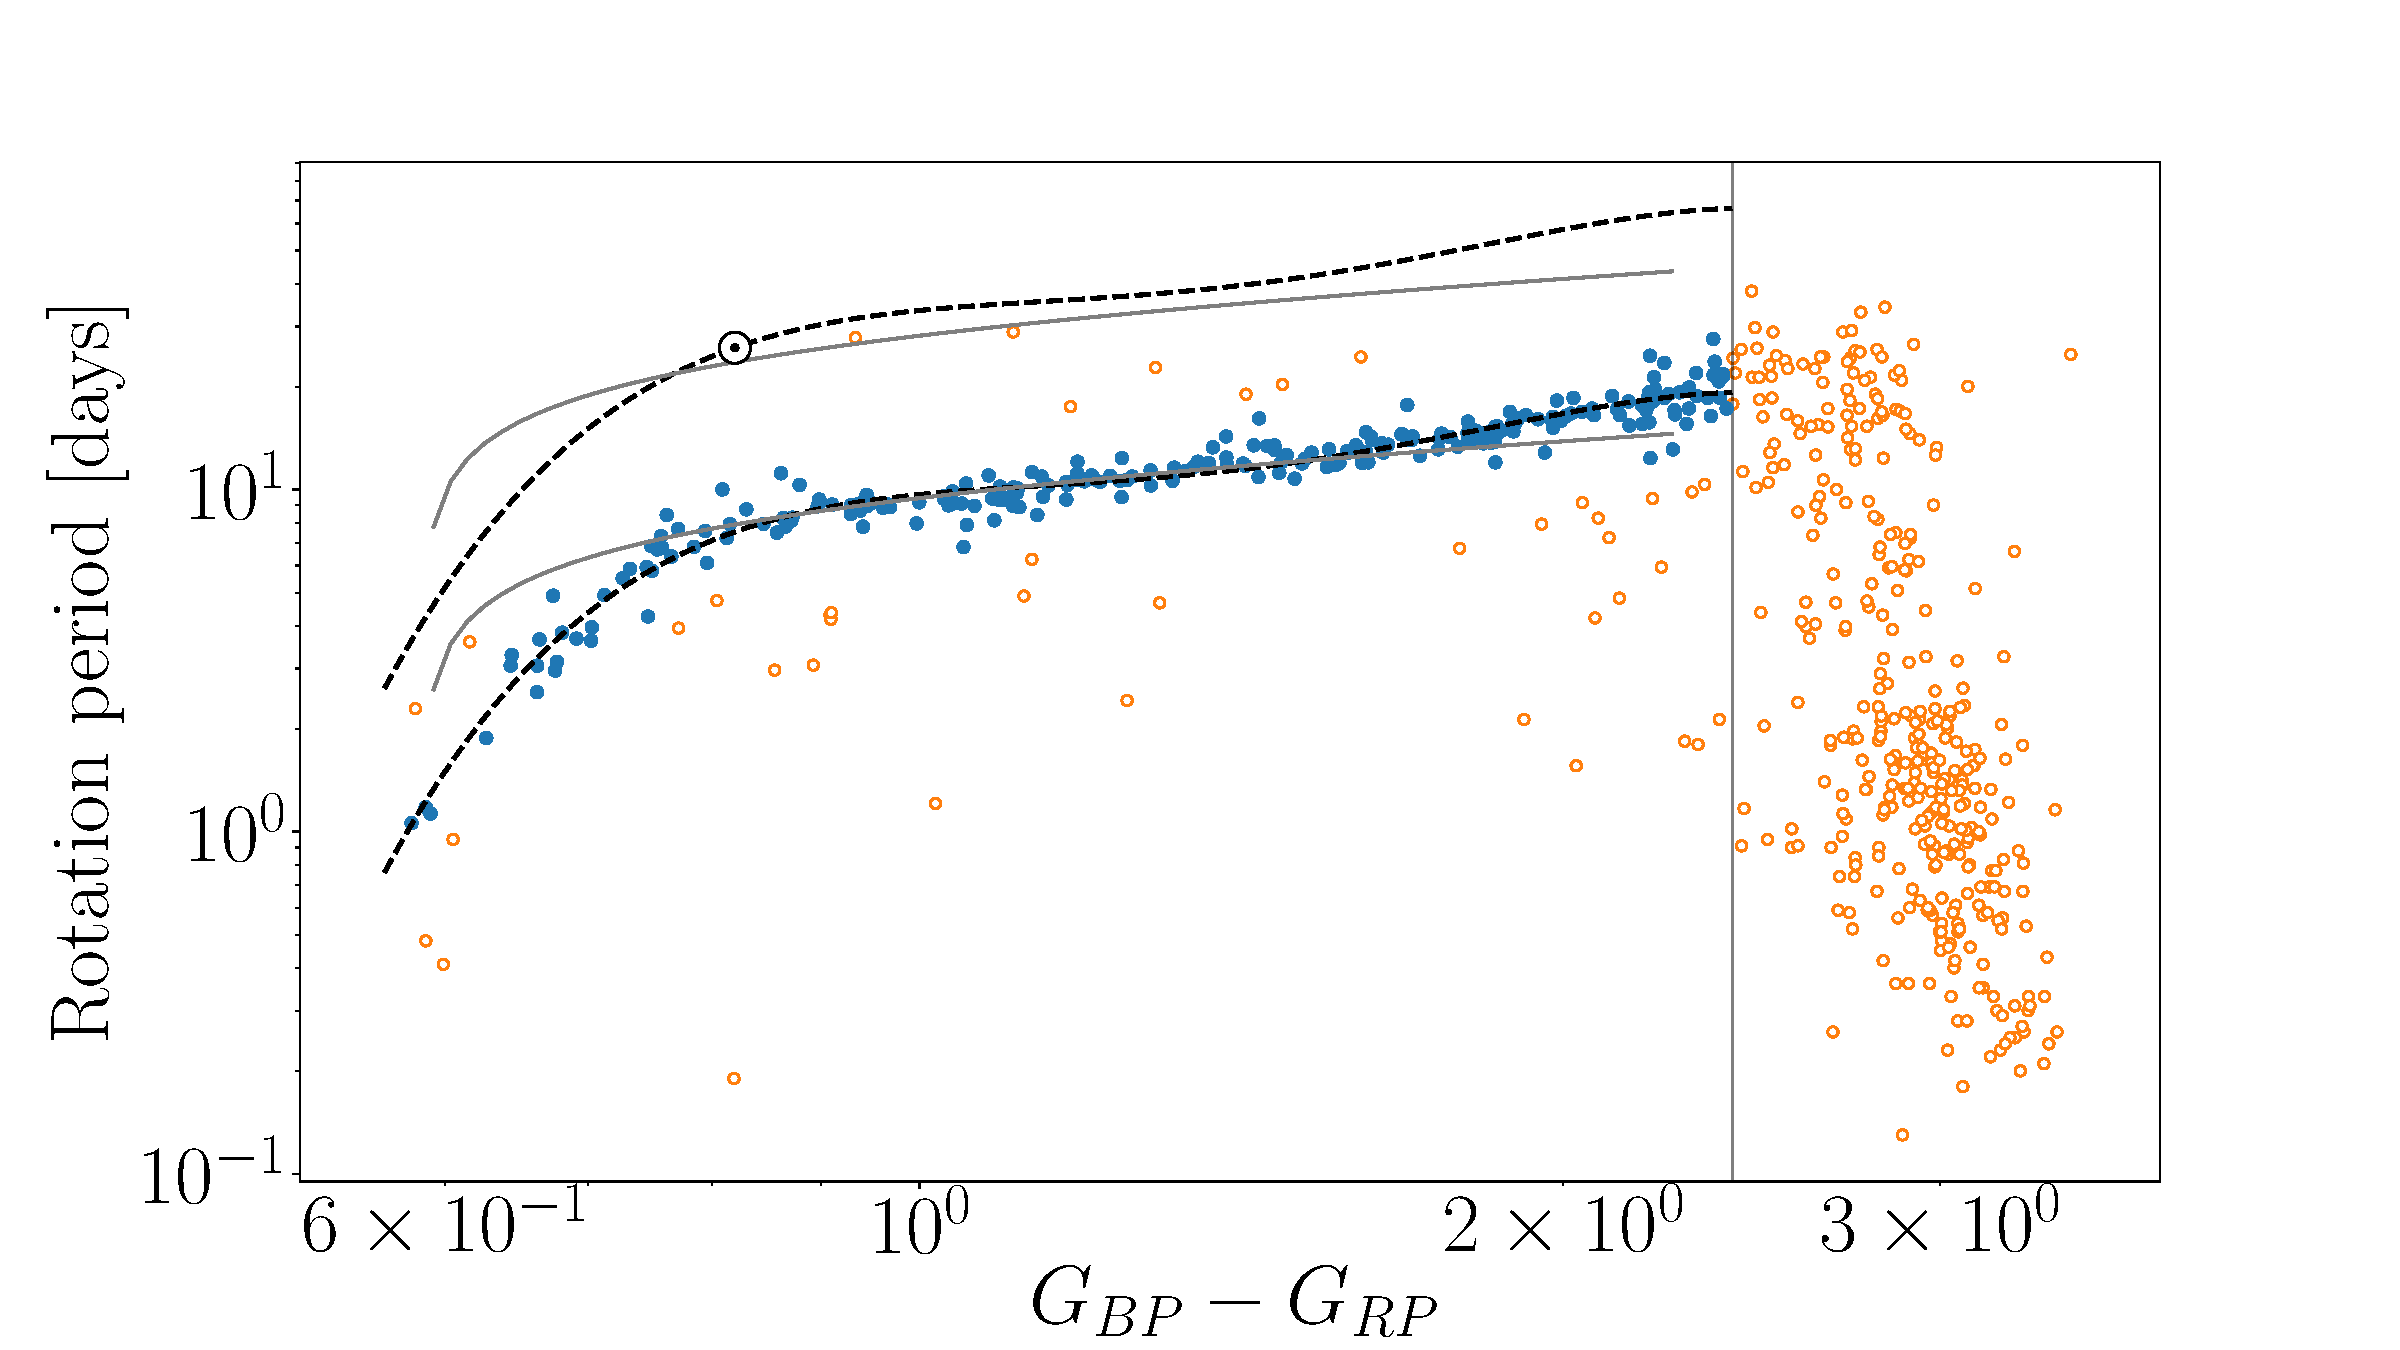
\includegraphics[width=1\textwidth]{with_angus_gyrochrones.pdf}
\label{fig:praesepe}
\end{figure}

\begin{figure}
  \caption{
    The unnormalized posterior PDFs over the ages of Praesepe stars inferred
    using an isochrone fitting method (orange) and a joint isochrone fitting
    and gyrochronology model (blue).
    MIST isochrones were used for isochrone fitting and the gyrochronology
    model is shown as solid grey lines in
    figure \ref{fig:praesepe} \citep{angus2015}.
    The black line shows the established age of Praesepe (650 Myrs).
    The blue posterior PDFs are more strongly peaked around the established
    age for Praesepe than the orange, indicating that gyrochronology is much
    more informative for these MS stars than isochrone fitting.
    \racomment{Still need to quantify the improvement}
}
  \centering
    \includegraphics[width=1\textwidth]{cluster_ages.pdf}
\label{fig:cluster_ages}
\end{figure}


% \begin{figure}
%   \caption{
%     The posterior PDFs over metallicity of Praesepe stars inferred using an
%     isochrone fitting method (orange) and a joint isochrone fitting and
%     gyrochronology model (blue).
%     The black line shows the established metallicity of Praesepe (citation).
%     The blue posterior PDFs are
% }
%   \centering
%     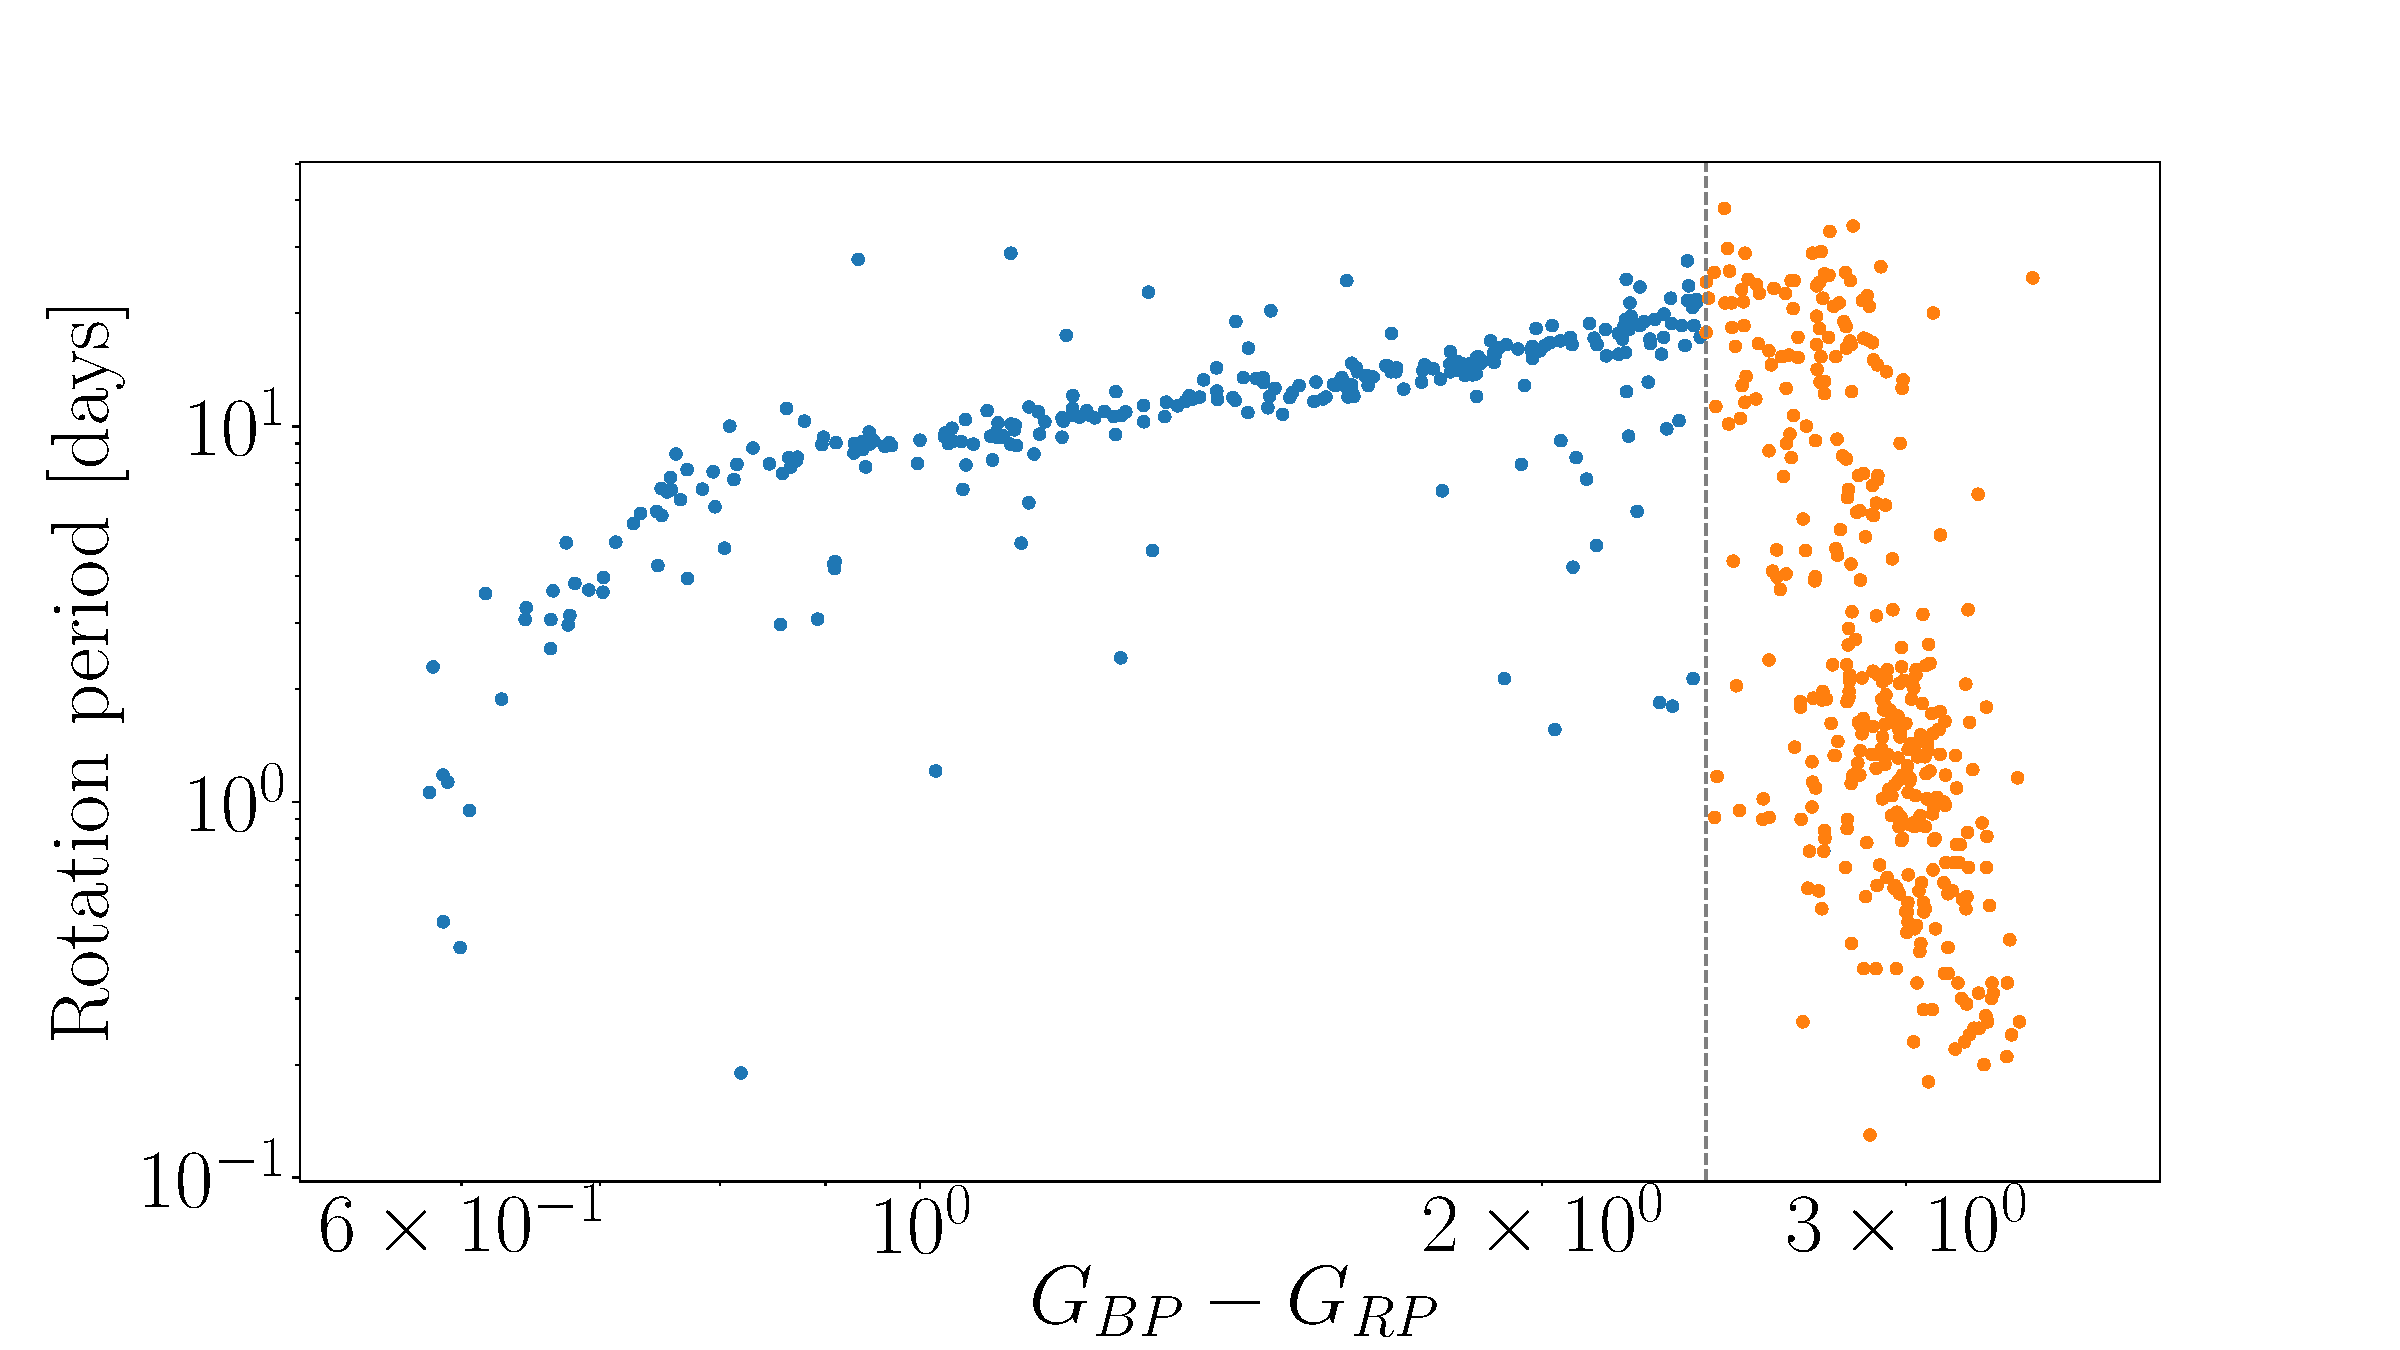
\includegraphics[width=1\textwidth]{praesepe.pdf}
% \label{fig:metallicity}
 % \end{figure}
